\documentclass[t,% Place text of slides at the (vertical) top of the slides
brazilian,% Brazilian Portuguese, FTW!
11pt,% Standard font size
aspectratio=169,% Aspect ratio 16:9 (widescreen)
table% xcolor option
]{beamer}

\setbeamercolor{footnote mark}{fg=red}

\usetheme{Boadilla}
\setbeamertemplate{navigation symbols}{}
\setbeamertemplate{frametitle continuation}{}
\setbeamertemplate{page number in head/foot}[framenumber]
\setbeamertemplate{enumerate items}[default]
\setbeamertemplate{itemize items}[circle]
\setbeamercovered{transparent}
\setbeamerfont{frametitle}{size=\normalsize}

\usepackage{babel}
\usepackage[utf8]{inputenc}
\usepackage[T1]{fontenc}
\usepackage{lmodern}

\usepackage{graphicx}
\setkeys{Gin}{keepaspectratio}

\usepackage{amssymb,amsfonts,amsmath}
\usepackage{mathtools}

\usepackage{siunitx}
\sisetup{locale = FR}

\usepackage{tikz}
\usetikzlibrary{calc}

\usepackage{pgffor}
\usepackage{etoolbox}

% \usepackage{colortbl}

\usepackage{tcolorbox}

\usepackage{pgfplots}
\pgfplotsset{compat=1.18}

\newcommand{\esima}{\textordfeminine }
\newcommand{\esimo}{\textordmasculine }

\newcommand{\vboxcorr}[2]{%
    \resizebox{!}{\totalheight-#1}{#2}%
}
\newcommand{\hboxcorr}[2]{%
    \resizebox{\width-#1}{!}{#2}%
}

\DeclareMathOperator{\arctg}{arctg}
\DeclareMathOperator{\sen}{sen}
\DeclareMathOperator{\arcsen}{arc sen}

\def\Disciplina{Fenômenos de Transporte}
\def\Professor{Rodrigo de Farias Gomes}
\def\Periodo{Período 2025.1}

\title{\Disciplina}
\author{\Professor}
\date{\Periodo}

\begin{document}

\begin{frame}
    \titlepage
\end{frame}

\begin{frame}{Informações gerais}
    \begin{itemize}
        \item Nome: {\fontfamily{augie}\selectfont Rodrigo de Farias Gomes}
        \item Telefone (somente mensagens): (92) 9 9405-1724
        \item E-mail: shpnft@gmail.com
        \item Sala: 201b, Bloco E (2\esimo{} pavimento)
    \end{itemize}
\end{frame}

\begin{frame}{Avaliação}
    \begin{itemize}
        \item A avaliação será na forma de 3 notas: \(N_1\), \(N_2\) e \(N_3\)
        \item A média dos exercícios escolares (\(ME\)) será dada por
            \[
                ME=\frac{N_1+N_2+N_3}{3}
            \]
        \item Se \(MEE \geq 8,0\), então a média final (\(MF\)) será igual à \(MEE\)
        \item Se \(MEE < 8,0\), então
            \[
                MF=\frac{2\times MEE+PF}{3}
            \]
            onde PF é a nota da \textbf{prova final}
        \item A prova final abordará o mesmo \textit{conteúdo} da última prova realizada
        \item Se \(MF \geq 5,0\) e a frequência em sala for maior que 75\%, o aluno está aprovado
    \end{itemize}
\end{frame}


\begin{frame}<1>[label=ementa]{Ementa de \Disciplina}
    \begin{itemize}
        \item Conceitos e definições fundamentais
        \item Conceitos de Fenômenos de Transporte e
            Analogia entre os Processos Difusivos Unidimensionais de
            Transferência de Movimento Linear, de Calor e de Massa
        \item Fundamentos da Estática dos Fluidos
        \item Descrição e Classificação de Escoamentos
        \item Introdução à Análise de Escoamentos na Formulação de Volume de Controle
        \item Introdução à Análise Diferencial de Escoamentos
        \item Introdução à Transferência de Calor
        \item Introdução à Condução Unidimensional de Calor em Regime Permanente
        \item Introdução à Condução de Calor em Regime Transiente
        \item Introdução à Transferência de Massa
    \end{itemize}
\end{frame}

\begin{frame}{Livro}
    \centering
    \vboxcorr{27pt}{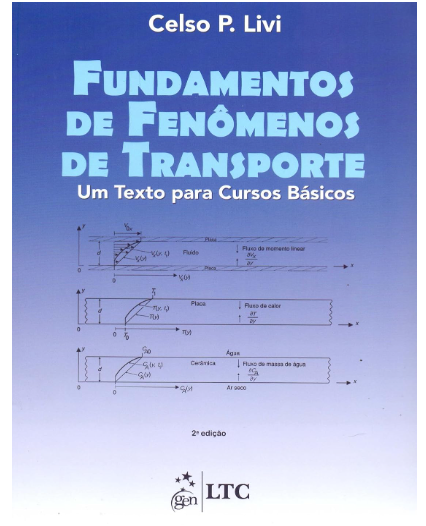
\includegraphics[height=\textheight]{images/Captura de tela de 2025-03-18 15-21-27.png}}
\end{frame}

\begin{frame}{Capítulos do Livro}
    \centering
    \vboxcorr{27pt}{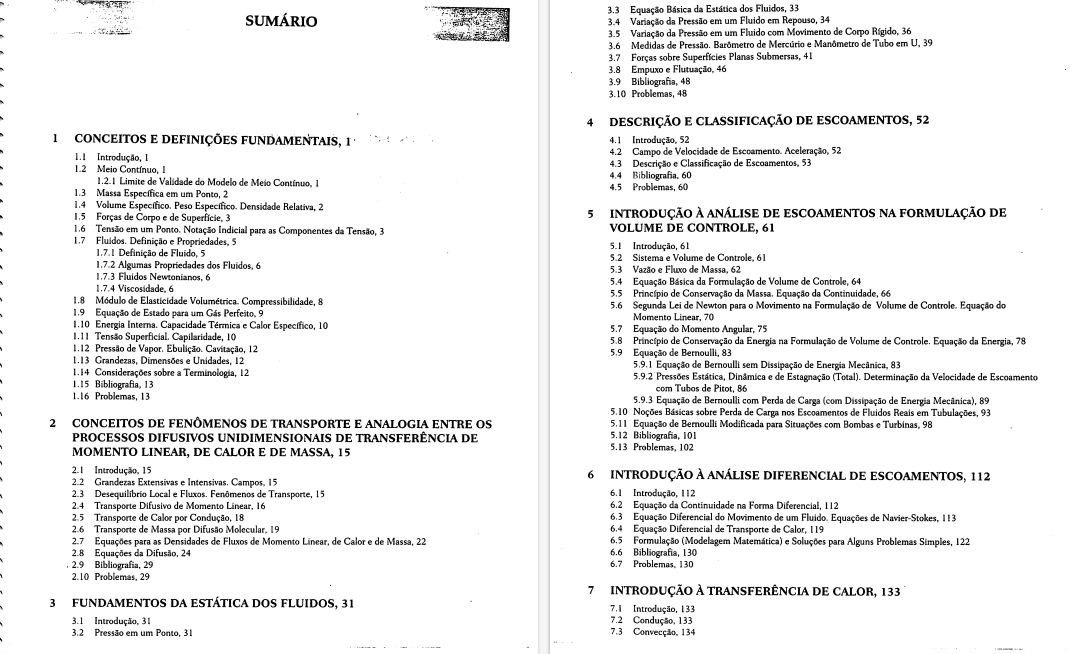
\includegraphics[height=\textheight]{images/Captura de tela de 2025-03-18 15-25-51.png}}
\end{frame}

\begin{frame}{Capítulos do Livro}
    \vboxcorr{27pt}{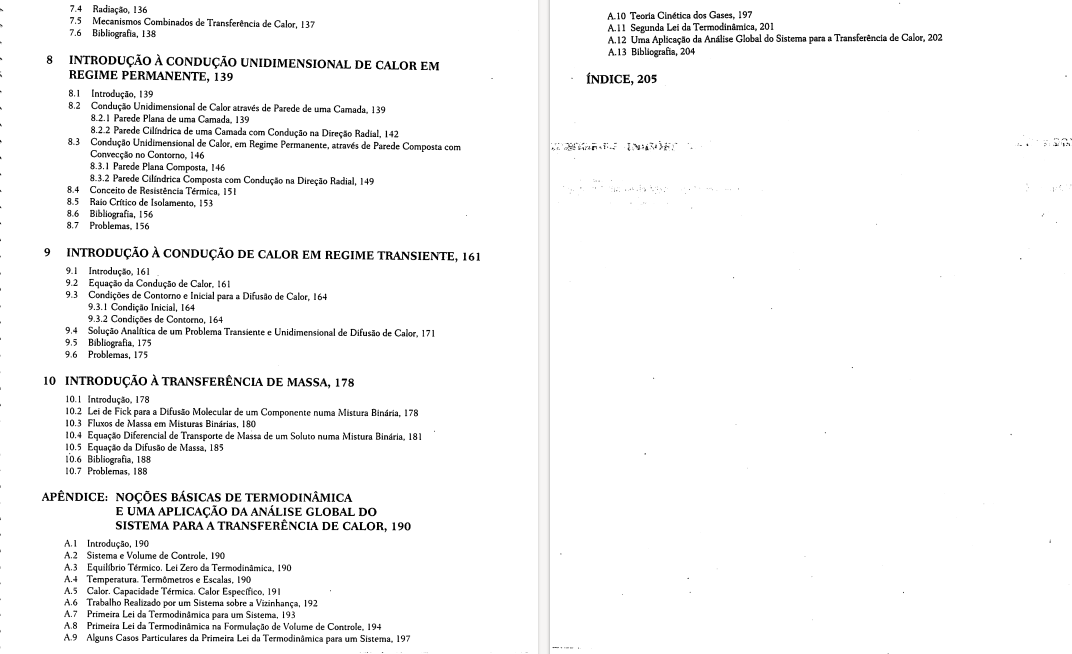
\includegraphics[height=\textheight]{images/Captura de tela de 2025-03-18 15-26-08.png}}
\end{frame}

\begin{frame}{Massa específica, volume específico e peso específico}
    \begin{itemize}
        \item Massa específica
            \[
                \rho = \lim_{\Delta V \to \delta V} \frac{\Delta m}{\Delta V} 
            \]
            onde:
            \begin{description}
                \item[\(\Delta m\)] é a massa contida no volume \(\Delta V\)
                \item[\(\delta V\)] é o menor volume onde seja válido o \textbf{modelo contínuo}
            \end{description}
        \item Volume específico
            \[
                v=\frac{1}{\rho}
            \]
        \item Peso específico
            \[
                \gamma = \rho g
            \]
    \end{itemize}
\end{frame}

\begin{frame}{Forças}
    \begin{itemize}
        \item Forças de corpo são aquelas que se manifestam através da interação com um campo e 
            atuam sem a necessidade de um contato entre as superfícies dos corpos.

            Exemplos: força peso, força elétrica, força magnética

            Forças de corpo são proporcionais ao volume dos corpos\footnote{Somente no caso de corpos uniformes}

        \item Forças de superfície são aquelas que atuam sobre um sistema através de contato com a fronteira do mesmo

            Exemplos: força de atrito, forças devido à \textit{pressão}

            Forças de superfície são proporcionais à área da superfície sobre a qual atuam
            \footnote{Somente no caso de corpos com superfícies uniformes}
    \end{itemize}
\end{frame}

\begin{frame}{Tensão e pressão}
    \begin{itemize}
        \item  A tensão é definida como a força por unidade de área aplicada a
            um corpo. Mas vimos em Física Geral II que pressão também é força
            por unidade de área. Qual a diferença?
        \item Pressão é uma grandeza \textbf{escalar} que só considera a componente \textit{normal} da força aplicada na superfície,
            enquanto a tensão é uma grandeza \textbf{tensorial} que considera todas as componentes
            \[
                \vec{\vec{T}}=
                \begin{bmatrix}
                    \sigma_{xx} & \tau_{xy} & \tau_{xz} \\ 
                    \tau_{yx} & \sigma_{yy} & \tau_{yz} \\
                    \tau_{zx} & \tau_{zy} & \sigma_{zz}
                \end{bmatrix}
            \]
            onde as \textbf{tensões normais} \(\sigma_{ii}\) são definidas como
            \[
                \sigma_{ii} = \lim_{\Delta A_i \to 0} \frac{\Delta F_i}{\Delta A_i}
            \]
            e as \textbf{tensões cisalhantes} (tangenciais) \(\tau_{ij}\) são definidas como
            \[
                \tau_{ij} = \lim_{\Delta A_i \to 0} \frac{\Delta F_j}{\Delta A_i}
            \]
    \end{itemize}
\end{frame}

\end{document}
